\documentclass{templateNote}
\usepackage{tcolorbox}
\usepackage{hyperref}
\usepackage{amsmath}
\usepackage{amssymb}
\usepackage{pdflscape}
\usepackage{soul}
\usepackage{media9}
\usepackage{adjustbox}
\usepackage{pdfpages}

\begin{document}

\imagenlogoU{img/LogoElNube.png}
\linklogoU{https://github.com/MarceloPazPezo}
\linkQRDoc{https://github.com/MarceloPazPezo/MyRepo/tree/main/Icinf/Semestre\%207/Sistemas\%20de\%20Información/Test\%201}
\titulo{Test 1}
\asignatura{Sistemas de Información}
\autor{
    \indent
    Marcelo \textsc{Paz}
    \\
    \indent
    Nicolas \textsc{Gómez}
    \\
    \indent
    Javier \textsc{Santander}
}
\portada
\margenes % Crear márgenes

\section{Sistemas de Información}
\begin{itemize}
    \item \textbf{Sistema:} Conjunto de partes que interactúan entre sí, para lograr un objetivo en común.
\end{itemize}
\begin{figure}[H]
    \centering
    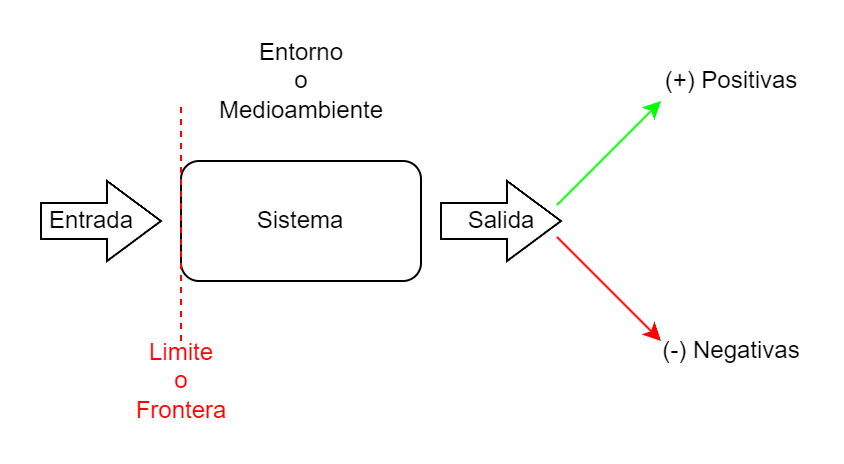
\includegraphics[width=0.9\textwidth]{diagramas/diagrama Sistema.png}
\end{figure}
Definiciones:
\begin{itemize}
    \item \textbf{Entrada:} Todo aquello que el sistema recoge de su entorno para cumplir con su objetivo.
    \item \textbf{Salida:} Todo aquello que el sistema entrega al entorno producto del cumplimiento de su objetivo.
    
    + Sistema se beneficia
    
    - Sistema no se beneficia
    
    Salida + > Salida -
\end{itemize}

\begin{itemize}
    \item \textbf{Sistema Abierto:} Es capaz de interactuar con el entorno por si solo.
    \item \textbf{Sistema Cerrado:} No es capaz de interactuar con el entorno por si solo.
    \item \textbf{Sinergia:} El todo es mas que las sumas de las partes. Las sumas de las partes cumplen un objetivo.
    \item \textbf{Conglomerado:} Conjunto de partes que no interactuán entre si.
    \item \textbf{Entropía:} Grado de desorden.
    \item \textbf{Dato:} Hecho conocido que no tiene valor.
    \item \textbf{Información:} Un dato al que se le agrega significado y utilidad.
    \item \textbf{Conocimiento Tácito:} Conocimiento que no se ve, como lo que esta en la mente de las personas.
    \item \textbf{Conocimiento Explícito:} Conocimiento que se puede ver, como textos o apuntes.
    \begin{itemize}
        \item Fácil de transmitir.
        \item Fácil de transpasar.
        \item Para transformar conocimiento tácito en explícito utilizando la documentación del conocimiento.
    \end{itemize}
    \item \textbf{Estrategia:} Es un camino a seguir para poder llegar al objetivo deseado.
    \item \textbf{Misión:} Razón de ser de la empresa.
    \item \textbf{Visión:} Sueño/Idea de llegar a ser.
    \item \textbf{Tecnologias de información:} Permiten desarrollar sistemas.
    \item \textbf{Recursos y capacidades:} El sistema no logra nada sin los recursos y capacidades.
    \item \textbf{Procesos:} Cosas que se hacen para convertir una entrada en salida.
    \item \textbf{Estructura:} Como se organiza.
    \item \textbf{Cultura:} Forma de hacer las cosas.
\end{itemize}

\begin{landscape}
    \begin{figure}[H]
        \centering
        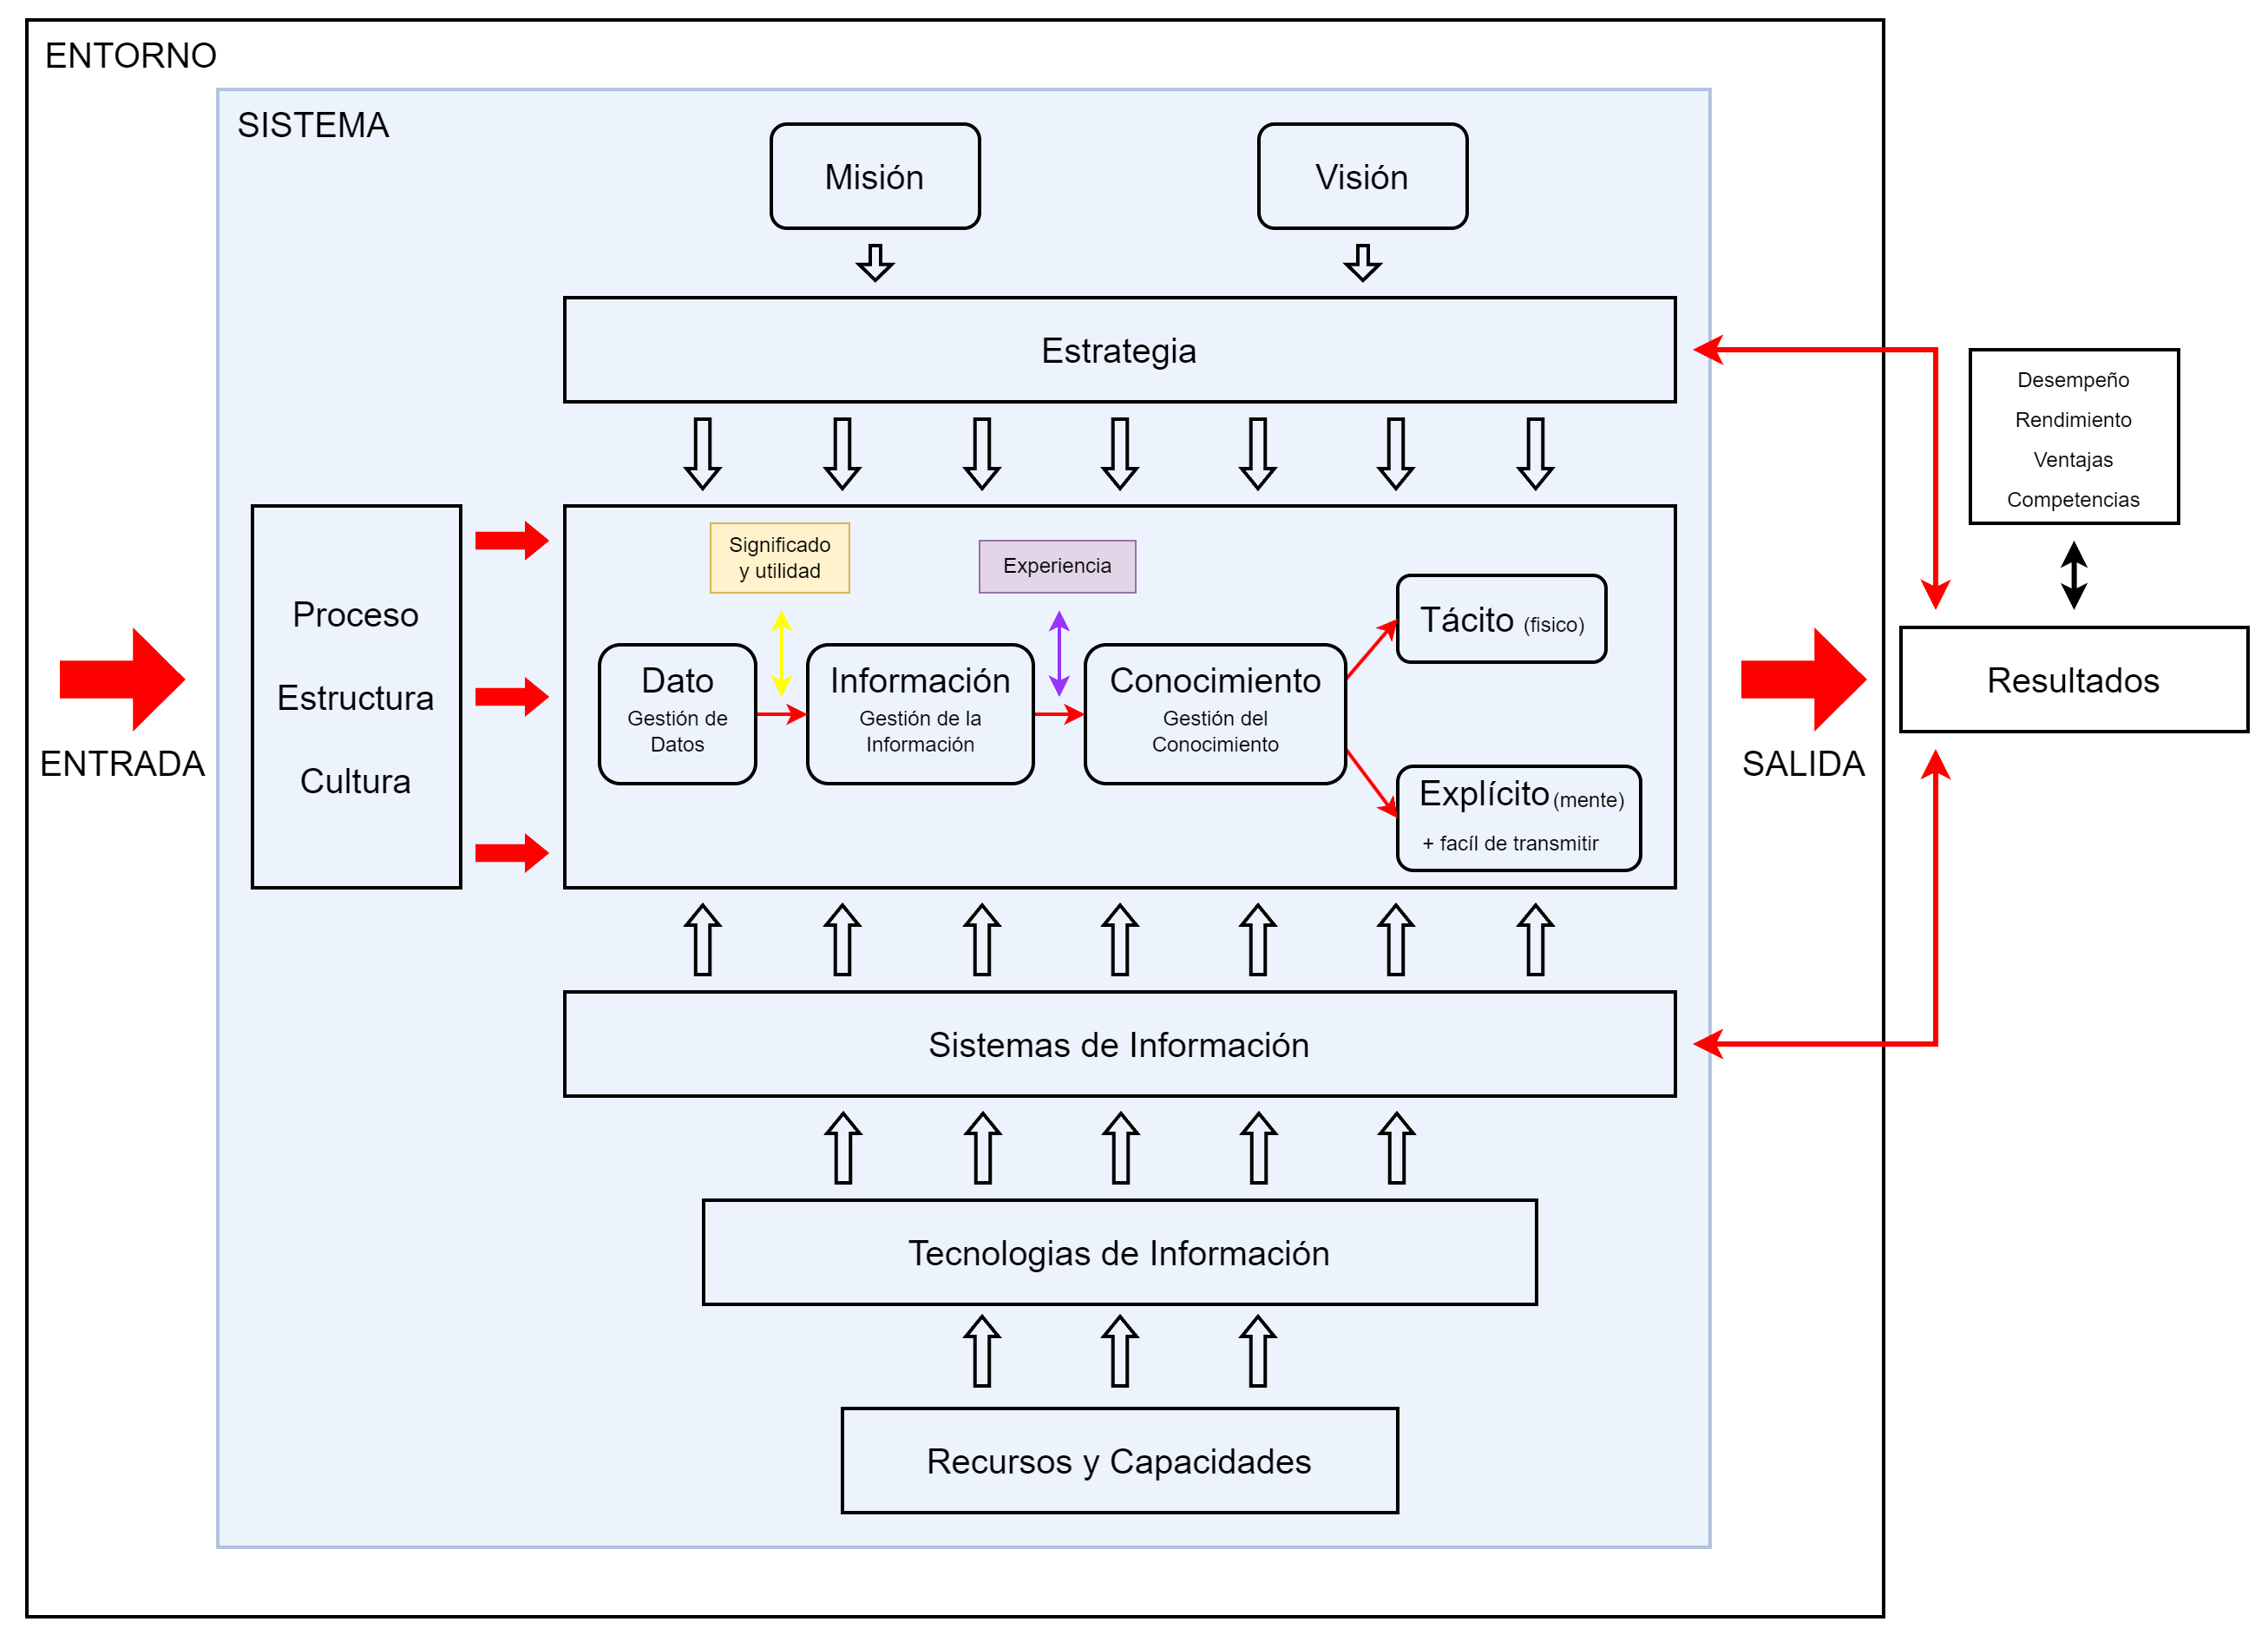
\includegraphics[width=1.35\textwidth]{diagramas/digramaCompleto.png}
    \end{figure}
\end{landscape}

\newpage
\subsection*{Explicación del Diagrama:}
\indent
La estrategia viene de la misión y visión de la organización (son permanentes). Los datos, información y conocimiento vienen de la estrategia. La gestión de estos es para la obtención de resultados. Los sistemas de información son una herramienta que perimte apoyar el manejo de los datos, información y conocimiento para la obtención de resultados.
Consecuentemente apoyan el logro de la estrategia para conseguir resultados. Los sistemas de información se crean con tecnologías de información las que se obtienen en base a recursos y capacidades. En la organización son llevados a cabo procesos, estructuras y culturas que segun los datos, información y conocimiento obtenido se manejara una estrategia y un sistema de información para poder lograr los resultados deseados. El diagrama igualmente cumple con la piramide de Anthony que muestra lo operativo en la base, lo táctico en el medio y lo estratégico en la punta.
\\
Los recursos y capacidades aparecieron como teoria a fines de los 80's. Antes de esto existia "Porter" que decia que aquellas organizaciones que se adapten mejor al entorno le irá mejor. Una persona complemento a "Porter" a mediados o fines de los 80's, diciendo que no es culpa del entorno sino de las condiciones de la empresa, en especifico de los recursos y capacidades de la organización.Teoria de recursos y capacidades: El que maneje mejor los recursos y capacidades le irá mejor que la competencia.
\textbf{Agradecimientos a Javier Santander}
\newpage
\section{Piramide de Anthony}
\indent
Siempre encontramos 3 niveles:
\begin{figure}[H]
    \centering
    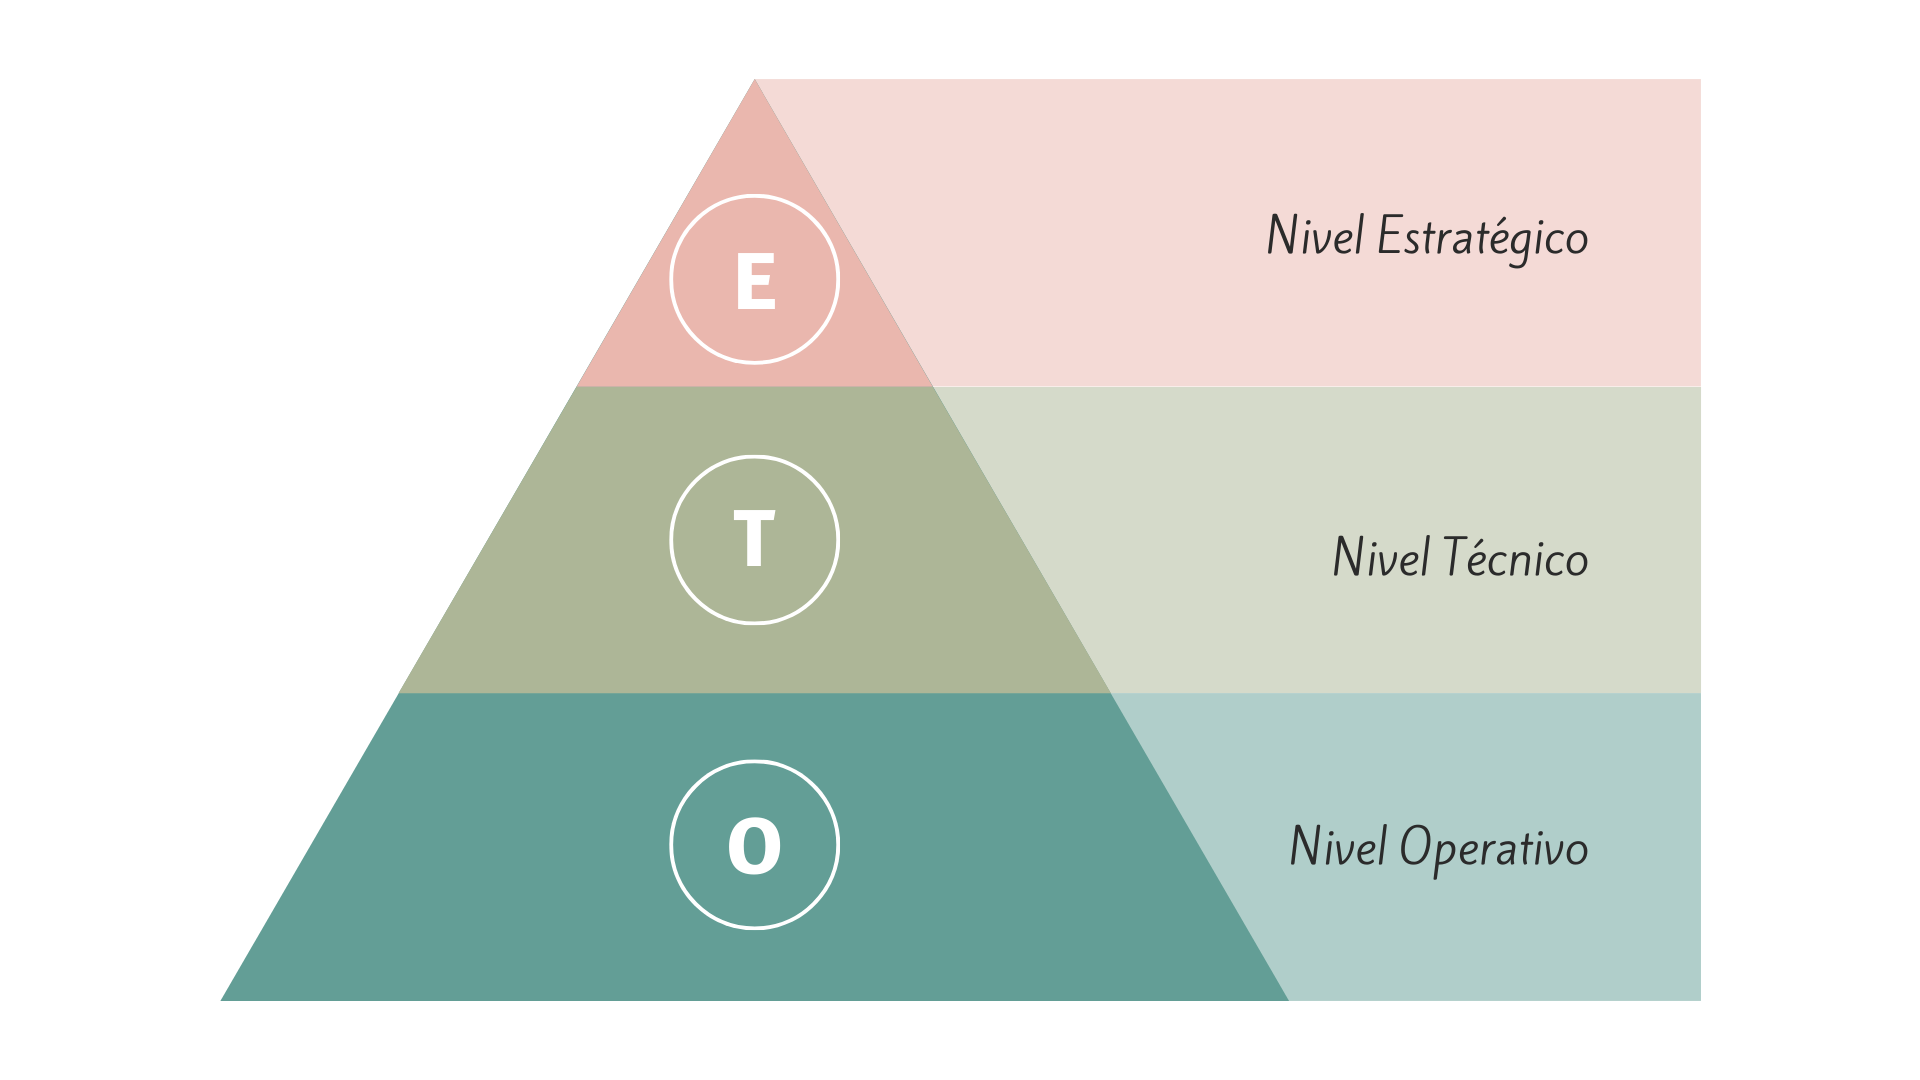
\includegraphics[width=0.7\textwidth]{img/PiramideAnthony.png}
    
    \textbf{Agradecimientos a Nicolas Gómez}
\end{figure}
\begin{itemize}
    \item \textbf{Nivel Estrategico:} Definición de Misión; Largo Plazo.
    \item \textbf{Nivel Táctico:} Control de gestión; Mediano Plazo.
    \item \textbf{Nivel Operativo:} Actividades rutinarias; No cambian; Corto Plazo.
\end{itemize}
\textbf{Explicación:} La piramide de Anthony. Ayuda a estructurar la información y/o las actividades de manera jerarquica. A menor nivel hay mas gente y las actividades son mas simples o rutinarias de hacer, y a mayor nivel hay menos personas y las decisiones son mas importantes por lo que hay un mayor plazo con el que se obtendran los resultados.
\section{Características de la Información}
\begin{figure}[H]
    \begin{center}
        \noindent\adjustbox{center}{
            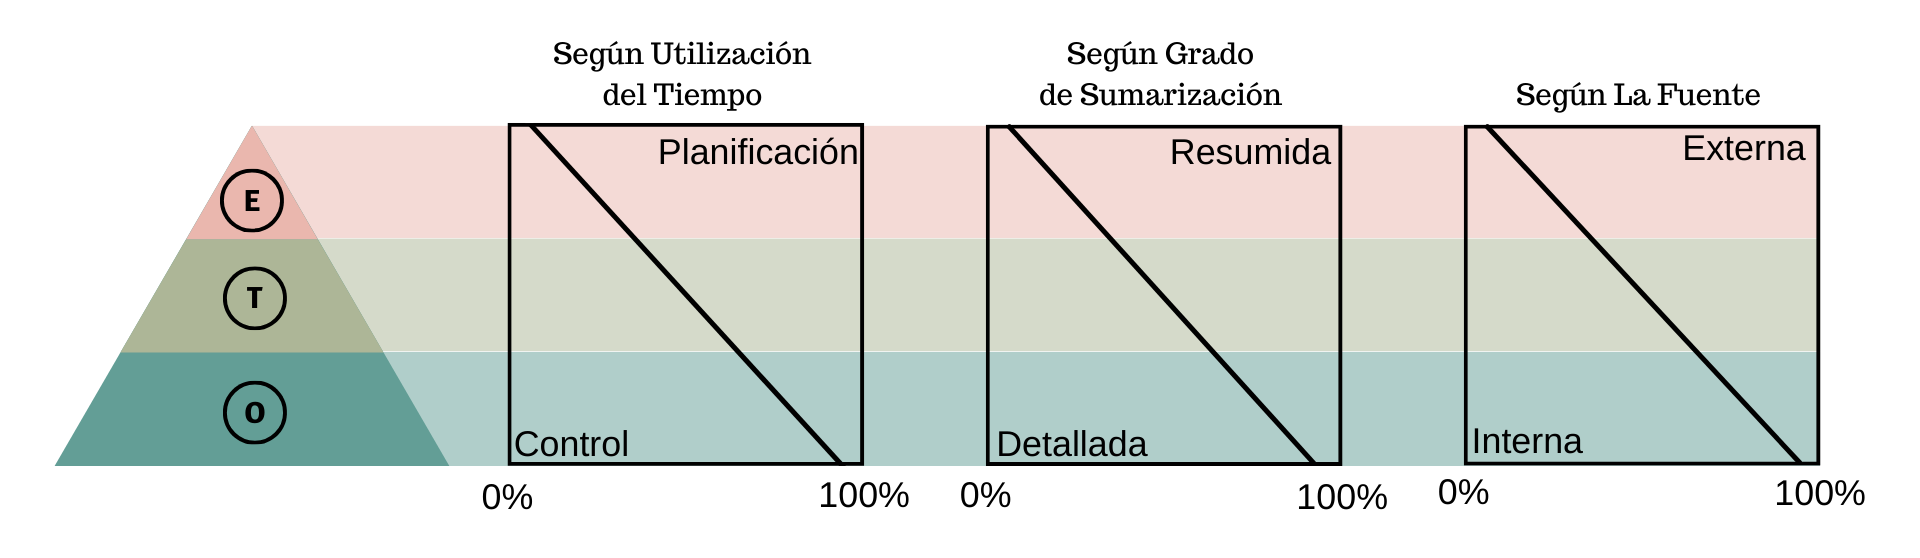
\includegraphics[width=1.2\textwidth]{img/PiramideAnthony2.png}
        }
        \textbf{Agradecimientos a Nicolas Gómez}
    \end{center}
\end{figure}
\begin{itemize}
    \item \textbf{Según la utilización del tiempo:}
    \begin{itemize}
        \item La mayor parte del tiempo arriba se usa la información para planificación y abajo para tener un mayor control. Al no partir desde el 0 se dice que no hay un gran control sin planificación ni tampoco hay una gran planificación sin un minimo de control.
        \item La información se utiliza la mayor cantidad del tiempo para actividades relacionadas con el control en el Operativo y mientras más se sube hay menor control y más planificación.
        \item * Entre más abajo sea el nivel la información se usará para actividades de mayor control y menor planificación. Entre más se suba en la piramide la información se utilizara para planificación.
    \end{itemize}

    \item \textbf{Según el grado de sumarización:}
    \begin{itemize}
        \item Mientras mas abajo en niveles estemos la información será más detallada y entre más se suba será más resumida. Ejemplo: El gerente pide algo de una página o un pequeño gráfico, no un informe de 100 páginas.
    \end{itemize}

    \item \textbf{Según la fuente:}
    \begin{itemize}
        \item En niveles más bajos se pedira información de fuentes internas para las actividades, entre más se suba será necesaria más de fuentes externas. Ejemplo: Una secretaria no tiene que saber sobre el dolar para la tarea que desempeña mientras que un gerente si.
    \end{itemize}
\end{itemize}

\begin{itemize}
    \item \textbf{Sistema de Información:} \hl{Conjunto formal de procesos} que operando sobre una \hl{colección de datos estructurados} recopila, elabora y distribuye (parte de) la información \hl{necesaria para la operación de dicha empresa} y para las actividades de \hl{dirección y control} correspondientes apoyando al menos en parte la toma de \hl{decisiones necesarias} para desempeñar las \hl{funciones y procesos} de acuerdo con la \hl{estrategia.}
    \begin{itemize}
        \item Un proceso es formal cuando esta bien definido, este proceso se puede estudiar.
        \item Un proceso es informal cuando no esta bien definido.
        \item Los datos estan estructurados según la necesidad de la empresa.
        \item Recopilación, elaboración y distribución $\rightarrow$ Sistema con entrada, proceso y salida.
    \end{itemize}

    \item \textbf{Planificación de recursos empresariales (E.R.P):} Es la planificación de recursos empresariales por la traducción al español. Son una clasificación de software que esta hecho de una forma dividida en modulos e integra las diferentes partes para mejorar la eficiencia. Son muy caros, son dificiles de implementar si se seguia un sistema previo con cierta cultura.

    \item \textbf{Plan informatico:} Estrategias de sistemas y tecnologias de información.
\end{itemize}

\section{Curva de Nolan}
\begin{figure}[H]
    \centering
    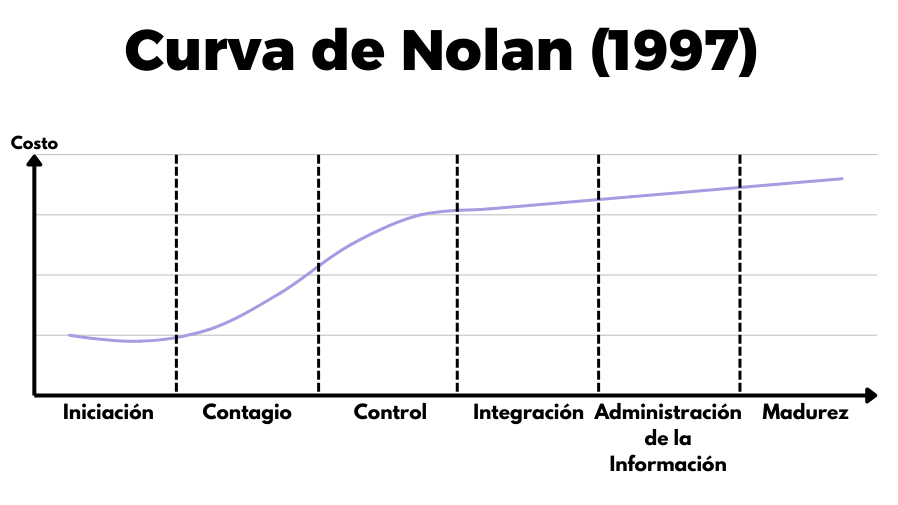
\includegraphics[width=0.7\textwidth]{img/CurvaDeNolan.png}
\end{figure}
\begin{itemize}
    \item Es una curva hecha en los años 1979 por Nolan y un amigo tratando originalmente mostrar como evolucionaba el costo en el tiempo. Actualmente, o para este ramo la usamos para observar como evolucionan los sistemas de información.
    
    \item \textbf{Inicialización:} Se empiezan a usar los primeros computadores, la gente que usaba estas maquinas eran vistos como raros y existian pocos usandolas.
    
    \item \textbf{Contagio:} Se dan cuenta que la gente que utiliza estos sistemas y tecnologias les beneficia y mejora la eficacia del trabajo. Todos empiezan a compra computadores por lo mismo.
    
    \item \textbf{Control:} Llega un momento en que los computadores, sistemas y tecnologias estan llegando a muchas personas y sin control por lo que se reduce su venta quedando solo para un grupo selecto.
    
    \item \textbf{Integración:} Se empieza a integrar de mejor manera los sistemas a las empresas para que exista comunicación entre areas y mejore la eficacia.
    
    \item \textbf{Administración de la información:} Los sistemas y la información son algo importante de la organización por lo que se le empieza a tomar más en serio considerandolos como recursos administrables.
    
    \item \textbf{Madurez:} No hay miedo a las tecnologias o sistemas.
\end{itemize}
*$Implementación \rightarrow Organización \rightarrow Dirección \rightarrow Control$
\newpage
\begin{landscape}
    \section*{Actualización de Curva de Nolan}
    \begin{figure}[H]
        \centering
        \vspace*{\fill}
        
        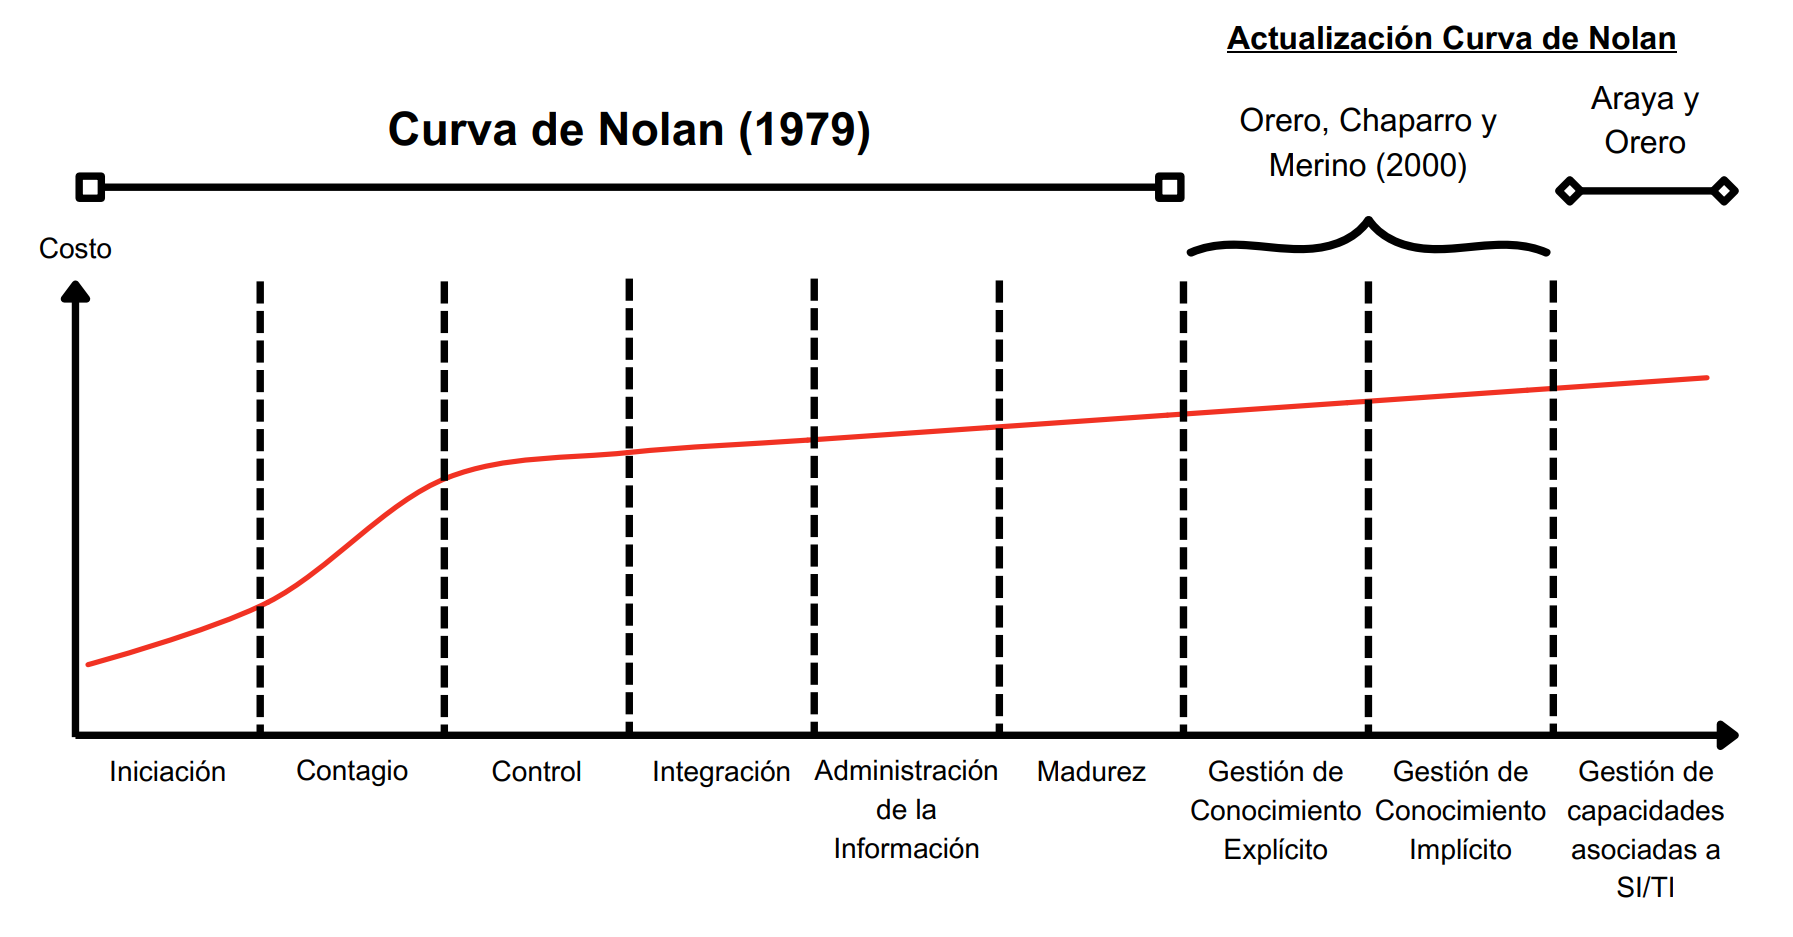
\includegraphics[width=1.3\textwidth,height=1.3\textheight,keepaspectratio]{img/CurvaDeNolanActualizada.png}
        \vspace*{\fill}
    \end{figure}
\end{landscape}
\newpage
\includepdf[pages={8,9}]{pdfs/Resumen.pdf}
\end{document}